\section{Joint input-scaling and dimension selection}
\label{sec:joint-selection}

The preceding experiment selects local dimension while fixing input
standardization. Since input scaling changes distances, partitions,
principal directions, and projected kernels, dimension selection alone
does not exhaust the declared geometry choices. We therefore conducted
a separately frozen experiment in the same representation-only architecture.
It uses fresh repetitions and evaluates both enrichment of a common
geometry and the performance of individually selected procedures.
The completed preceding experiment remains unchanged; its terminal
observations are neither fitting or validation data for this study
nor pooled with this cohort. All 256 tasks and the independent
computational audit have completed.

\paragraph{Candidate geometry and unchanged decoder.}
Let $T_s$ denote an input transform fitted on the A histories and let
$c$ be a native local-dimension cap. The ordered grid is
\[
 \mathcal S\times\mathcal C
 =\{\text{standard},\text{min--max},\text{tanh}\}
   \times\{1,2,4,8,12\}.
\]
Standardization uses A population means and standard deviations.
Min--max uses A extrema, maps nonconstant A coordinates to $[-1,1]$,
and does not clip subsequent queries. An exactly constant A coordinate
is mapped to zero. The tanh transform is
$\tanh((x_k-\mu_{A,k})/\sigma_{A,k})$, with the inherited
small-scale rule and no subsequent input restandardization.
For every pair, one A-fitted bank supplies all four arms. The
partition sizes, reference limit, kernel construction, blockwise
standardization and radial maps, and ridge grid remain as in
Section~\ref{sec:softstate-study}. Thus G and P retain their exact
shared-prefix identities inside each candidate. Scaling can change
the bank across candidates; it is not assumed to preserve the same
geometry or numerical information.

For arm $a$, horizon $h$, scaler $s$, and cap $c$, B selects the ridge
penalty $\widehat\lambda_{a,h}(s,c)$ from the same five penalties.
The geometry score is
\begin{equation}
 Q_a(s,c)=\frac{1}{3}\sum_{h\in\{1,4,12\}}
 \frac{\MSE_{B,h}\!\left(\widehat f_{a,h,s,c,
       \widehat\lambda_{a,h}(s,c)}\right)}
 {\max\{\Var_A(Y_h),10^{-12}\}}.
 \label{eq:joint-selection-score}
\end{equation}
All coefficients, input transforms, and feature transforms are fitted
on A. Selected states are retained without a subsequent A+B refit.
C is diagnostic only and D is terminal evaluation only. Ties choose
the first scaler in the displayed order and then the first ascending
cap; penalty ties likewise choose the first grid entry.

\paragraph{Structural and complete-procedure comparisons.}
In the joint shared-bank view, P minimizes $Q_P(s,c)$ and all arms
use that bank with their own penalties. In the joint independent
view, each arm minimizes its own $Q_a(s,c)$. These views respectively
test enrichment of a selected common representation and the
performance of a complete tuned procedure. Neither compares a
K-selected geometry against a control arbitrarily held to P's bank.
Two standard-only views restrict the identical cached fits to
$s=\text{standard}$, selecting either with P or separately for each
arm. No additional models are fitted for these references. They
isolate the effect of expanding the scaling menu on the same fresh
cohort. Inclusion of the standard-only candidates guarantees a
weakly smaller selected B score for each arm in the independent
view and for P in the shared view. It gives no such guarantee for
the other arms on P's selected bank, or for any terminal loss.

\paragraph{Fixed cohort and primary comparisons.}
The experiment has 32 new independent repetitions and 256 task suites,
with the same laws, noise levels, histories, horizons, and A/B/C/D
allocation as the preceding study. A new master seed and an explicit
predecessor-stream exclusion check preceded generation. The protocol,
source, analysis, and independent audit were frozen and the source
published as commit \texttt{8e025027} before production preparation.
The fitted-state roster was sealed before D generation and the
terminal forecasts were sealed before target release and scoring.

One six-contrast primary family contains the four shared-bank
questions from the preceding study and two direct tests of joint
tuning: independently joint-selected K versus independently
dimension-selected standard-only K, with a 3\% nonlinear superiority
margin and a 5\% linear noninferiority margin. Repetition aggregates
remain the inferential units. The upper bound for a margin-adjusted
paired difference is
$\overline d+t_{1-0.05/6,31}s_d/\sqrt{32}$; a criterion is established
only when this bound is negative. Independent K/R comparisons and
law, noise, horizon, and selection-frequency breakdowns are
descriptive. The finite search does not globally optimize every
geometry parameter or establish autonomous soft-state dynamics.

\begin{table}[tbp]
\centering\small
\setlength{\tabcolsep}{4pt}
\begin{tabular}{@{}lllrrc@{}}
\toprule
Panel & Contrast & Criterion & Gain (\%) & $U$ & Met \\
\midrule
Nonlinear & $P/G$ & 3\% superiority & 68.69 & -0.0587852 & Yes \\
Nonlinear & $K/P$ & 3\% superiority & 8.86 & -0.00144862 & Yes \\
Nonlinear & $K/R$ & 3\% superiority & -0.9186 & 0.00119423 & No \\
Linear & $K/P$ & 5\% noninferiority & -1.26 & -0.0305374 & Yes \\
Nonlinear & $K_{\mathrm{joint}}/K_{\mathrm{standard}}$ & 3\% superiority & 0.0727 & 0.000901116 & No \\
Linear & $K_{\mathrm{joint}}/K_{\mathrm{standard}}$ & 5\% noninferiority & -0.2491 & -0.0417521 & Yes \\
\bottomrule
\end{tabular}

\caption{Six primary comparisons in the joint-selection experiment.
The first four use P's selected common bank; the last two compare
independently selected K procedures on the same cohort. Gain is
$100(1-\overline L_{\rm candidate}/\overline L_{\rm reference})$,
so a negative value means higher candidate loss. $U$ is the
simultaneous upper bound for the margin-adjusted paired difference;
the criterion is established only if $U<0$. Nonlinear criteria
require 3\% superiority and linear criteria allow 5\% noninferiority.}
\label{tab:joint-primary}
\end{table}

\paragraph{Shared geometry: useful enrichment without K/R superiority.}
Table~\ref{tab:joint-primary} establishes four of the six primary
criteria. In the shared-bank nonlinear population, P improves G
by \JSGainPG\% and K improves P by \JSGainKP\%; both simultaneous
bounds establish their 3\% margins. K's loss is
\JSRelativeLossChangeKR\% higher than R's, so the K/R superiority
criterion is not established. The corresponding nonlinear means
are \JSLossSharedNonlinearK\ for K and
\JSLossSharedNonlinearR\ for R. In the linear population, K's
loss is \JSRelativeLossChangeLinearKP\% higher than P's, while
the bound establishes the specified 5\% noninferiority margin.
Thus the position and conditional KAHM-enrichment findings persist
on fresh repetitions after expanding the geometry menu, but this
experiment supplies no KAHM-specific advantage over the matched RBF
construction.

\paragraph{Complete K procedure: little aggregate gain from the larger menu.}
Independently joint-selected K has nonlinear mean loss
\JSLossIndependentNonlinearK, versus
\JSLossStandardIndependentNonlinearK\ for independently
dimension-selected standard-only K. The point improvement is only
\JSGainJointKNonlinear\%, and the simultaneous bound does not
establish the prescribed 3\% superiority margin. On the linear
population, joint K's loss is
\JSRelativeLossChangeJointKLinear\% higher, while its bound
establishes 5\% noninferiority. The two direct tuning criteria
therefore do not jointly establish improved nonlinear performance
with linear noninferiority. This is a same-cohort comparison of selected
procedures; its small point difference is neither a guaranteed
benefit from extra choices nor evidence of equivalence.

\begin{figure}[tbp]
\centering
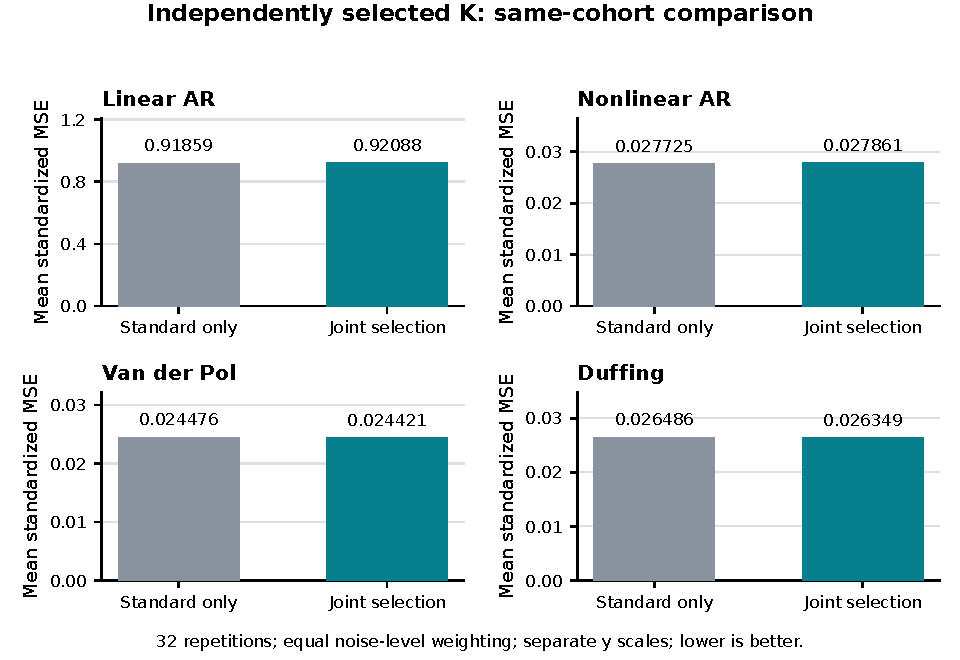
\includegraphics[width=0.88\linewidth]{generated/joint_selection/independent_K_joint_vs_standard.pdf}
\caption{Independently selected K with standard-only and joint
input-scaling menus. Each mean equally weights the two noise
conditions within each of 32 repetitions. All panels use a zero
origin but have separate vertical scales; lower loss is better.
The law-level comparisons are descriptive, with no uncertainty
intervals shown. Small oscillator gains accompany a nonlinear-AR
penalty, giving only a \JSGainJointKNonlinear\% aggregate nonlinear
gain under the prespecified weighting.}
\label{fig:joint-scaling}
\end{figure}

The law-level point comparisons in Figure~\ref{fig:joint-scaling}
show small gains for Van der Pol and Duffing and higher loss for
nonlinear autoregression. Joint K has lower nonlinear aggregate
loss in 15 of the 32 repetition pairs and higher loss in 17.
Independent K/R is also descriptive: K's nonlinear mean
\JSLossIndependentNonlinearK\ exceeds R's
\JSLossIndependentNonlinearR. These summaries do not replace
the six primary decisions. Selection frequencies, all four views,
resource records, and audit scope are retained in
the joint-selection section of the Supplementary Studies.
\FloatBarrier
